\documentclass[a4paper, 12pt]{article}
\usepackage[utf8]{inputenc}
\usepackage{myshortcuts}
\usepackage{a4wide}
\usepackage[version=4]{mhchem}
\usepackage{physics}
\usepackage{csquotes}
\usepackage{enumitem}
\usepackage{etoolbox}
\usepackage{multirow}
\usepackage[british]{babel}
\usepackage[labelfont=bf]{caption}
\usepackage[caption=false]{subfig}
\usepackage[style=numeric,backend=biber,sorting=none]{biblatex}
\usepackage[separate-uncertainty=true, multi-part-units=single]{siunitx}

\allowdisplaybreaks

\sisetup{detect-all = true}
\addbibresource{mysources.bib}

\DeclareSIUnit \px {px}

\title{
\textbf{Physics Internal Assessment}\\
\bigskip
What effect does varying the diameter of a thin wire have on the width of diffraction fringes produced?
}
\author{}
\date{}

\begin{document}
\maketitle

\section{Rationale}
The laws of optics govern how our eyes perceive the world around us. 
Reflection, refraction, and diffraction are common phenomena in our everyday life, occurring with not only sound waves but also electromagnetic waves. 
Of particular interest to me is the phenomenon of optical diffraction, which in the IB physics textbook is described as \autocite[151]{textbook}: 
\begin{quote}
``[...] when waves pass through a narrow gap or slit, or when their path is partly blocked by an object, the waves spread out [...].''    
\end{quote}

In class, we investigated the diffraction patterns when monochromatic laser light passes through a single \textit{slit}. 
The single slit diffraction experiment is rather well known as it demonstrates the wave properties of light. 
Yet, what happens when an \textit{object} obstructs the path of light is only very briefly mentioned with an equation of the position of the first diffraction minimum in topic 12 \autocite[495]{textbook}. 
My background research showed that it is possible to measure the diameter of thin wires with optical diffraction \autocite{wire_measurement}. 
This leads to my research question: 
what effect does varying the diameter of a thin wire have on the width of diffraction fringes?

In addition, I wish to improve on the procedure of the single slit diffraction experiment.
Many inaccuracies arose from directly measuring the width of the central bright fringe with a ruler on the screen.
The screen was a white piece of paper taped on the wall, which moved easily when the ruler was placed on it. 
Moreover, identifying the precise positions of the minima with the naked eye was not easy on a screen without visual scales.
Instead, an RGB photo analysis will overcome these issues.
Photographing the diffraction patterns from a distance does not move the screen, and as such does not introduce additional systematic errors.
Digital analysis of the photos can then be carried out using the computer vision library OpenCV \autocite{opencv_library}, allowing the locations of the minima to be determined with greater precision.
It should be noted that whilst the width of a bright fringe is measured in pixels on the photo, it suffices to use a millimetre paper as the screen to convert such width to SI units --- this facilitates calculations in the rest of the investigation.

\section{Background Theory}
\begin{figure}[H]
\centering
\minipage{0.5\textwidth}
\centering
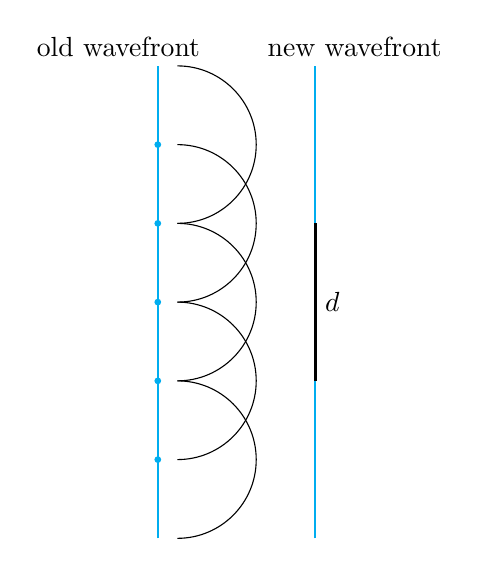
\begin{tikzpicture}
    \draw[cyan, thick] (0, -3) -- (0, 3);
    \filldraw[cyan] (0, -2) circle (1pt);
    \filldraw[cyan] (0, -1) circle (1pt);
    \filldraw[cyan] (0, 0) circle (1pt);
    \filldraw[cyan] (0, 1) circle (1pt);
    \filldraw[cyan] (0, 2) circle (1pt);
    \draw (0.25, -3) arc (-90:90:1cm);
    \draw (0.25, -2) arc (-90:90:1cm);
    \draw (0.25, -1) arc (-90:90:1cm);
    \draw (0.25, 0) arc (-90:90:1cm);
    \draw (0.25, 1) arc (-90:90:1cm);
    \draw[cyan, thick] (2, -3) -- (2, 3);
    \draw[very thick] (2, -1) -- (2, 1);
    \node[right] at (2, 0) {$d$};
    \node[above] at (-0.5, 3) {old wavefront};
    \node[above] at (2.5, 3) {new wavefront};
\end{tikzpicture}
\caption{Light before reaching the wire}
\label{fig:theory_before}
\endminipage\hfill
\minipage{0.5\textwidth}
\centering
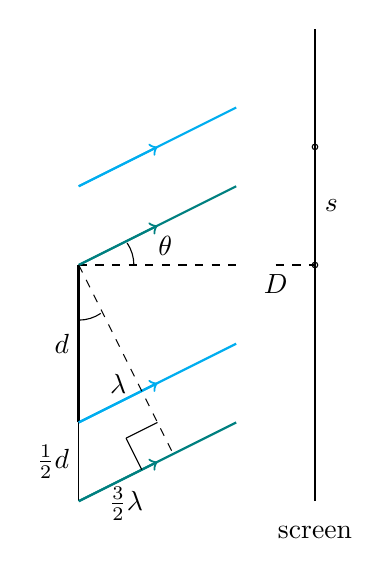
\begin{tikzpicture}
    \draw[very thick] (0, -1) -- (0, 1);
    \draw (0, -1) -- (0, -2);
    \node[left] at (0, 0) {$d$};
    \draw[dashed] (0, 1) -- (2, 1);
    \draw (0.7, 1) arc (0:34:0.5cm);
    \node[above] at (1.1, 1) {$\theta$};
    \draw[cyan, thick, ->] (0, 2) -- (1, 2.5);
    \draw[cyan, thick] (0, 2) -- (2, 3.0);
    \draw[teal, thick, ->] (0, 1) -- (1, 1.5);
    \draw[teal, thick] (0, 1) -- (2, 2.0);
    \draw[cyan, thick, ->] (0, -1) -- (1, -0.5);
    \draw[cyan, thick] (0, -1) -- (2, 0.0);
    \draw[teal, thick, ->] (0, -2) -- (1, -1.5);
    \draw[teal, thick] (0, -2) -- (2, -1.0);
    \draw[dashed] (0, 1) -- (1.2, -1.4);
    \draw (1.0, -1) -- (0.6, -1.2);
    \draw (0.6, -1.2) -- (0.8, -1.6);
    \draw (0, 0.3) arc (-90:-56:0.5cm);
    \node[above] at (0.5, -0.75) {$\lambda$};
    \node[left] at (0, -1.5) {$\frac{1}{2} d$};
    \node[below] at (0.6, -1.7) {$\frac{3}{2}\lambda$};
    \draw [dashed] (2.5, 1) -- (3, 1);
    \draw[thick] (3, -2.0) -- (3, 4.0);
    \node[below] at (3, -2.2) {screen};
    \draw (3, 2.5) circle (1pt);
    \draw (3, 1) circle (1pt);
    \node[right] at (3, 1.75) {$s$};
    \node[below] at (2.5, 1.0) {$D$}; 
\end{tikzpicture}
\caption{Light after reaching the wire}
\label{fig:theory_after}
\endminipage\hfill
\end{figure}
Let us consider the light waves immediately after being obstructed by the thin wire. 
Huygen's principle states that every point on a wavefront emits wavelets, i.e., rays that start in phase and propagate in all directions. 
The wavefront when the laser light hits the wire of diameter $d$ is shown in \cref{fig:theory_before}. 

Moreover, as shown in \cref{fig:theory_after}, assuming that the diameter $d$ of the wire is negligible compared to the distance $D$ from the wire to the screen, we can consider the rays hitting the screen at the same position as practically parallel. 
The rays travelling at an angle of $\theta$ relative to the centre line hit the screen at a distance of $s$ from the centre.

However, there is a difference in the path lengths of these rays. \Cref{fig:theory_after} shows two light rays interfering destructively: 
there is a path difference of $\frac{3}{2}\lambda$ between the two rays in teal.
We hypothesise that similarly, each ray beneath the wire interferes destructively with a ray above the wire since the path difference is an integer multiple of $\frac{1}{2}\lambda$.
In this case, the minimum occurs at $\sin\theta = \lambda / d$.
More generally, the positions of all the minima are given by
\[\sin\theta = \frac{n \lambda}{d},\ n \in \Z^*.\]
With $s \ll D$, we also have $\sin\theta = \tan\theta = s / D$. 
We then obtain
\[
s = n \frac{\lambda D}{d},
\]
and as a consequence, each bright fringe measures
\begin{align}
    \Delta s = \frac{\lambda D}{d}\label{eq:hypothesis}
\end{align}
wide except for the central bright fringe which has double this width.

We now verify this hypothesised relationship between $\Delta s$ and $d$ with experimental data.

\section{Variables}
\subsection*{Independent variable}
$d$, diameter of the wire. Manufacturer's values (in \si{\um}): $38, 50, 76, 100, 120, 150$.
\begin{figure}[H]
    \centering
    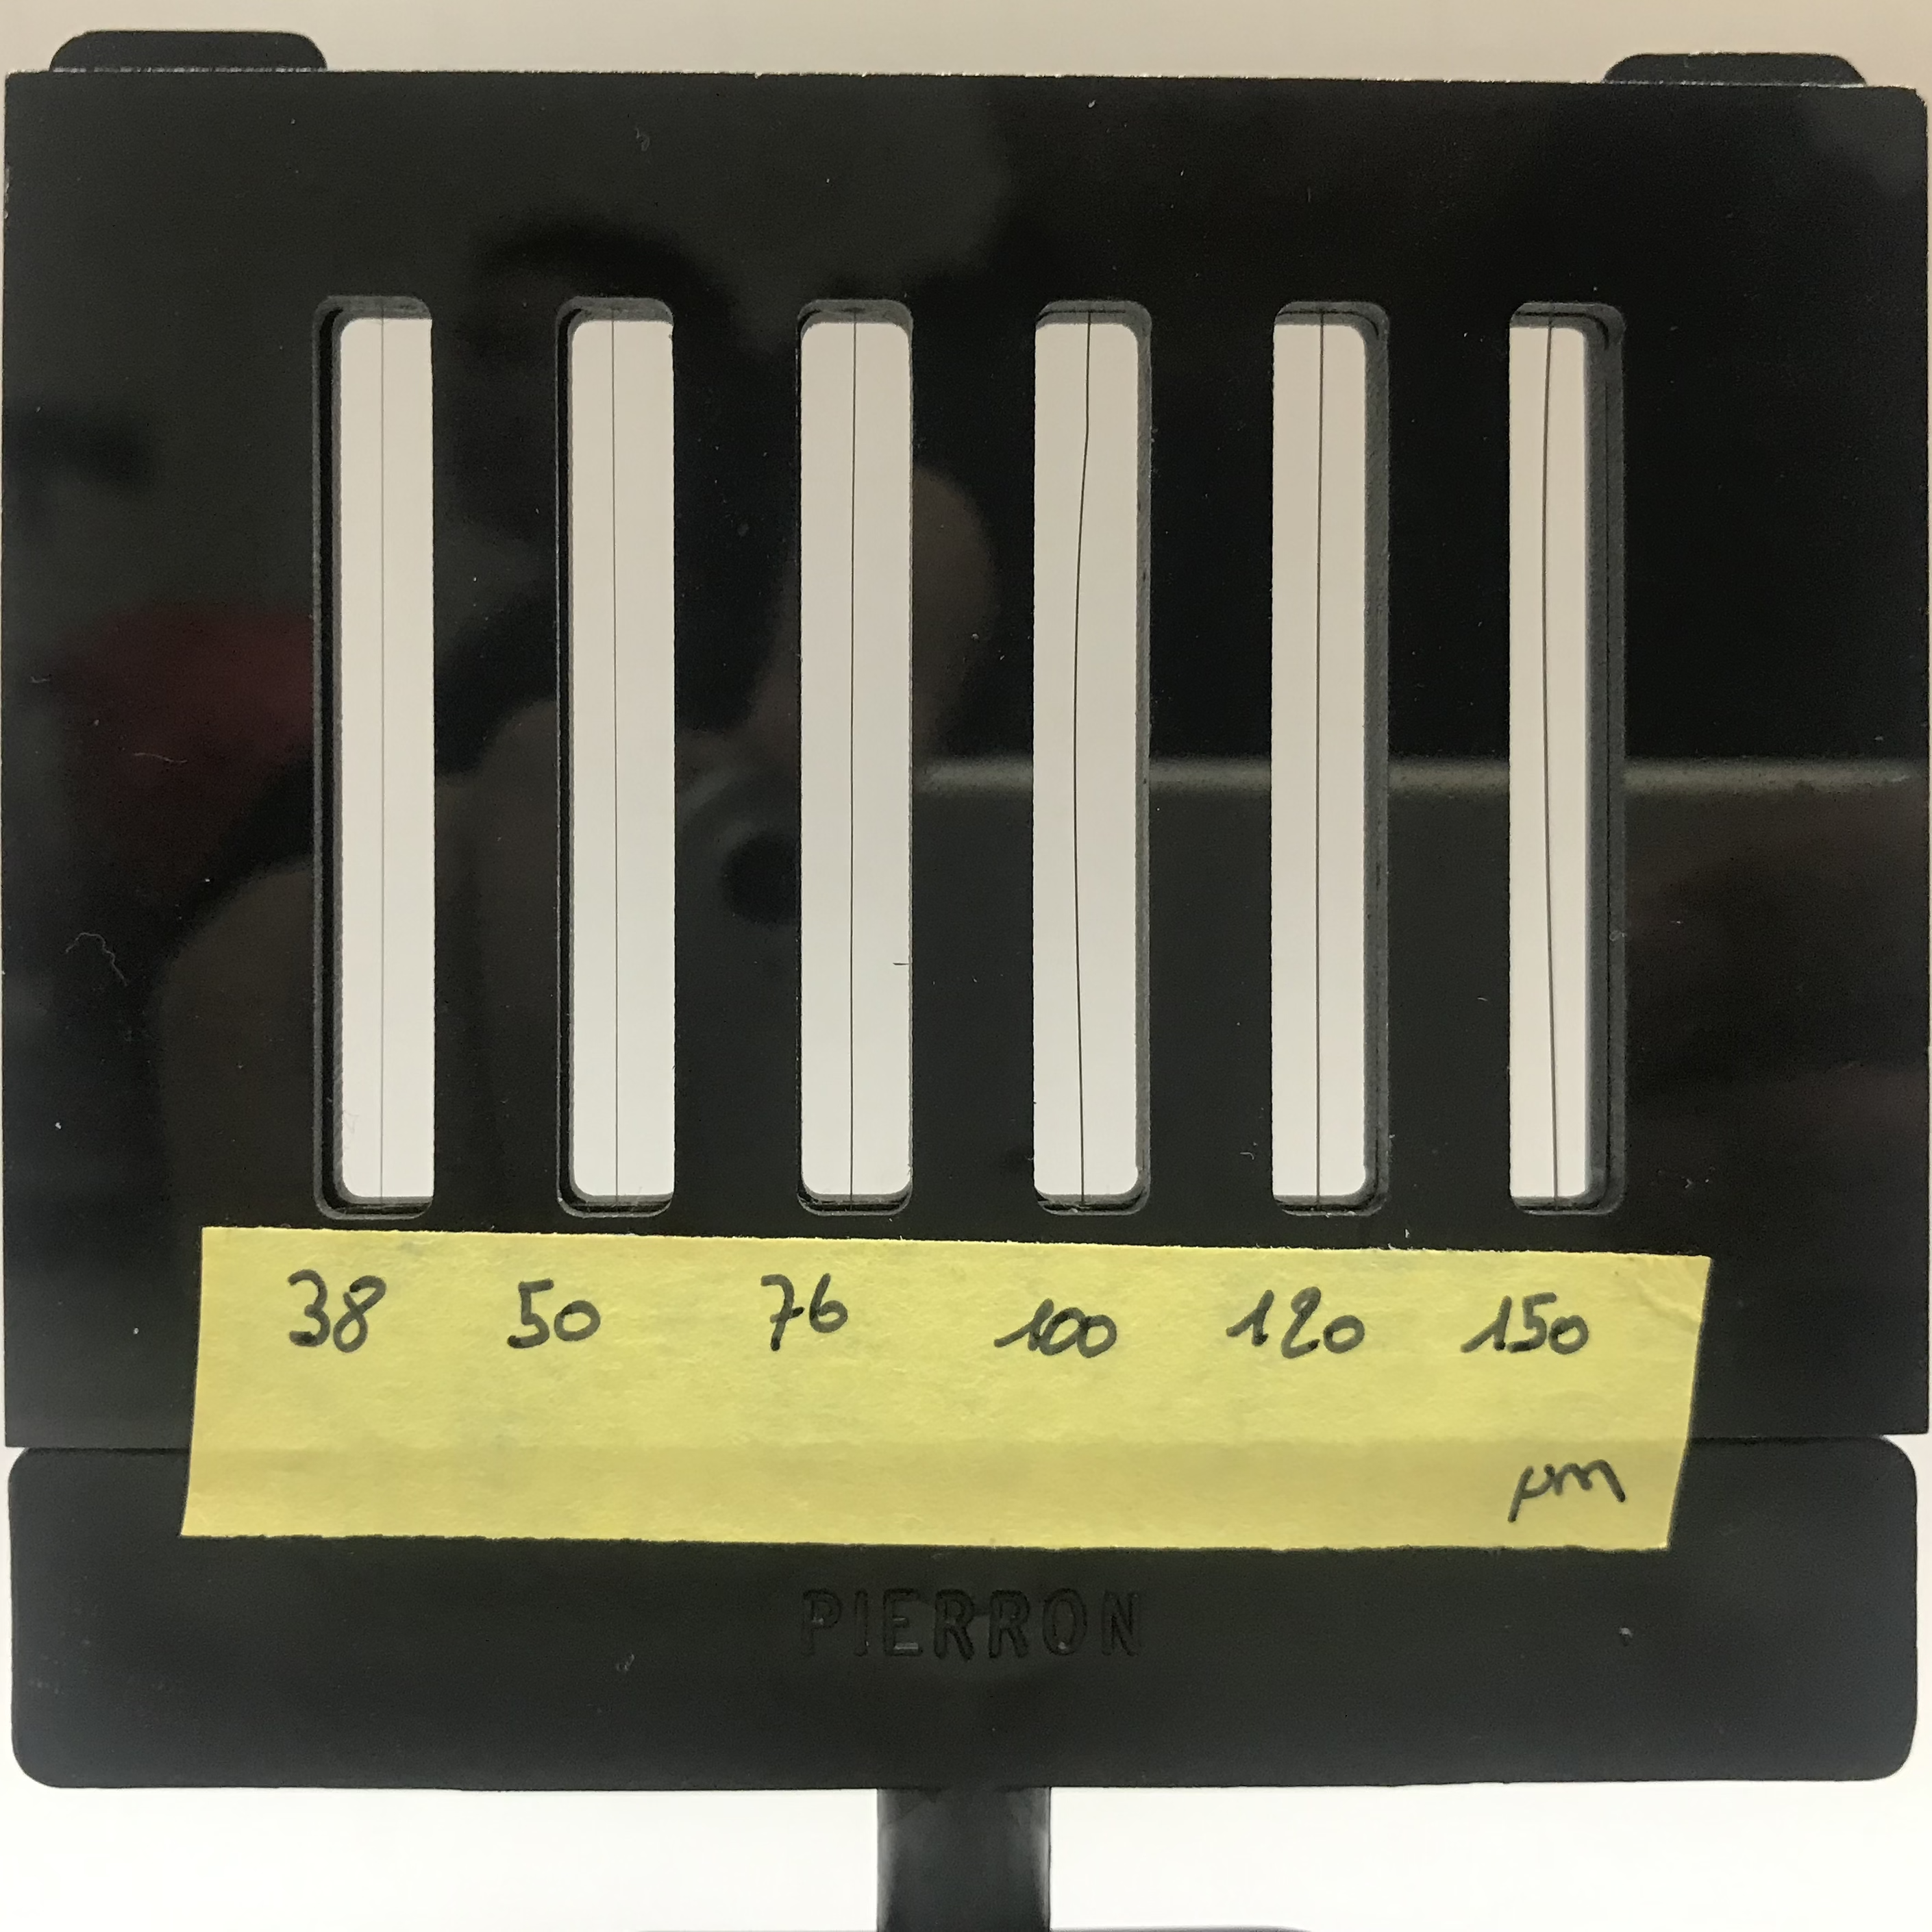
\includegraphics[width=0.4\textwidth]{img/wires}
    \caption{Diameters of wires used in the experiment}
    \label{fig:wires}
\end{figure}

\subsection*{Dependent variable}
$\Delta s$, width of bright fringes. Measured against a piece of millimetre paper in \si{\mm} with computer program that I wrote \autocite{py_extract}.

\subsection*{Controlled variables}
\begin{itemize}
\itemsep 0em
    \item $\lambda$, wavelength of laser light --- \SI{650+-10}{\nm} \autocite{laser-specs}
    \item $D$, distance from the wire to the screen --- \SI{2.250+-0.010}{\m}, with a tape measure
    \item Angle and position from which the photos are taken
\end{itemize}
$\lambda$ and $D$ are controlled because they are part of \cref{eq:hypothesis}, the hypothesised relationship between $\Delta s$ and $d$. 
The photographing is also controlled to avoid errors in $\Delta s$.

\section{Method}
To minimise the impact of ambient lighting on the diffraction pattern observed, I carried out the experiment in a dark room. 
Since the pupil then dilates to improve vision by allowing more light into the eye, special care was taken to avoid shining the laser beam or its reflection into the eye. 
Measures to prevent eye damages included ensuring that no one else is in the same room and not pointing the laser on reflective surfaces.

\begin{enumerate}
\itemsep 0.2em
    \item Fix the end of the tape measure between the table and the wall, and extend the tape in a straight line up to the other end of the table.
    \item Using the reading from the measuring tape, place the wire stand at a distance of \SI{2.250+-0.010}{\m} away from the wall. \label{step:place-stand}
    \item Set up the laser diode behind the stand so that the wire obstructs the laser beam by padding the diode with one or two thick books from below if needed (see \cref{fig:setup}). Turn on the laser diode. \label{step:place-laser}
\begin{figure}[H]
    \centering
    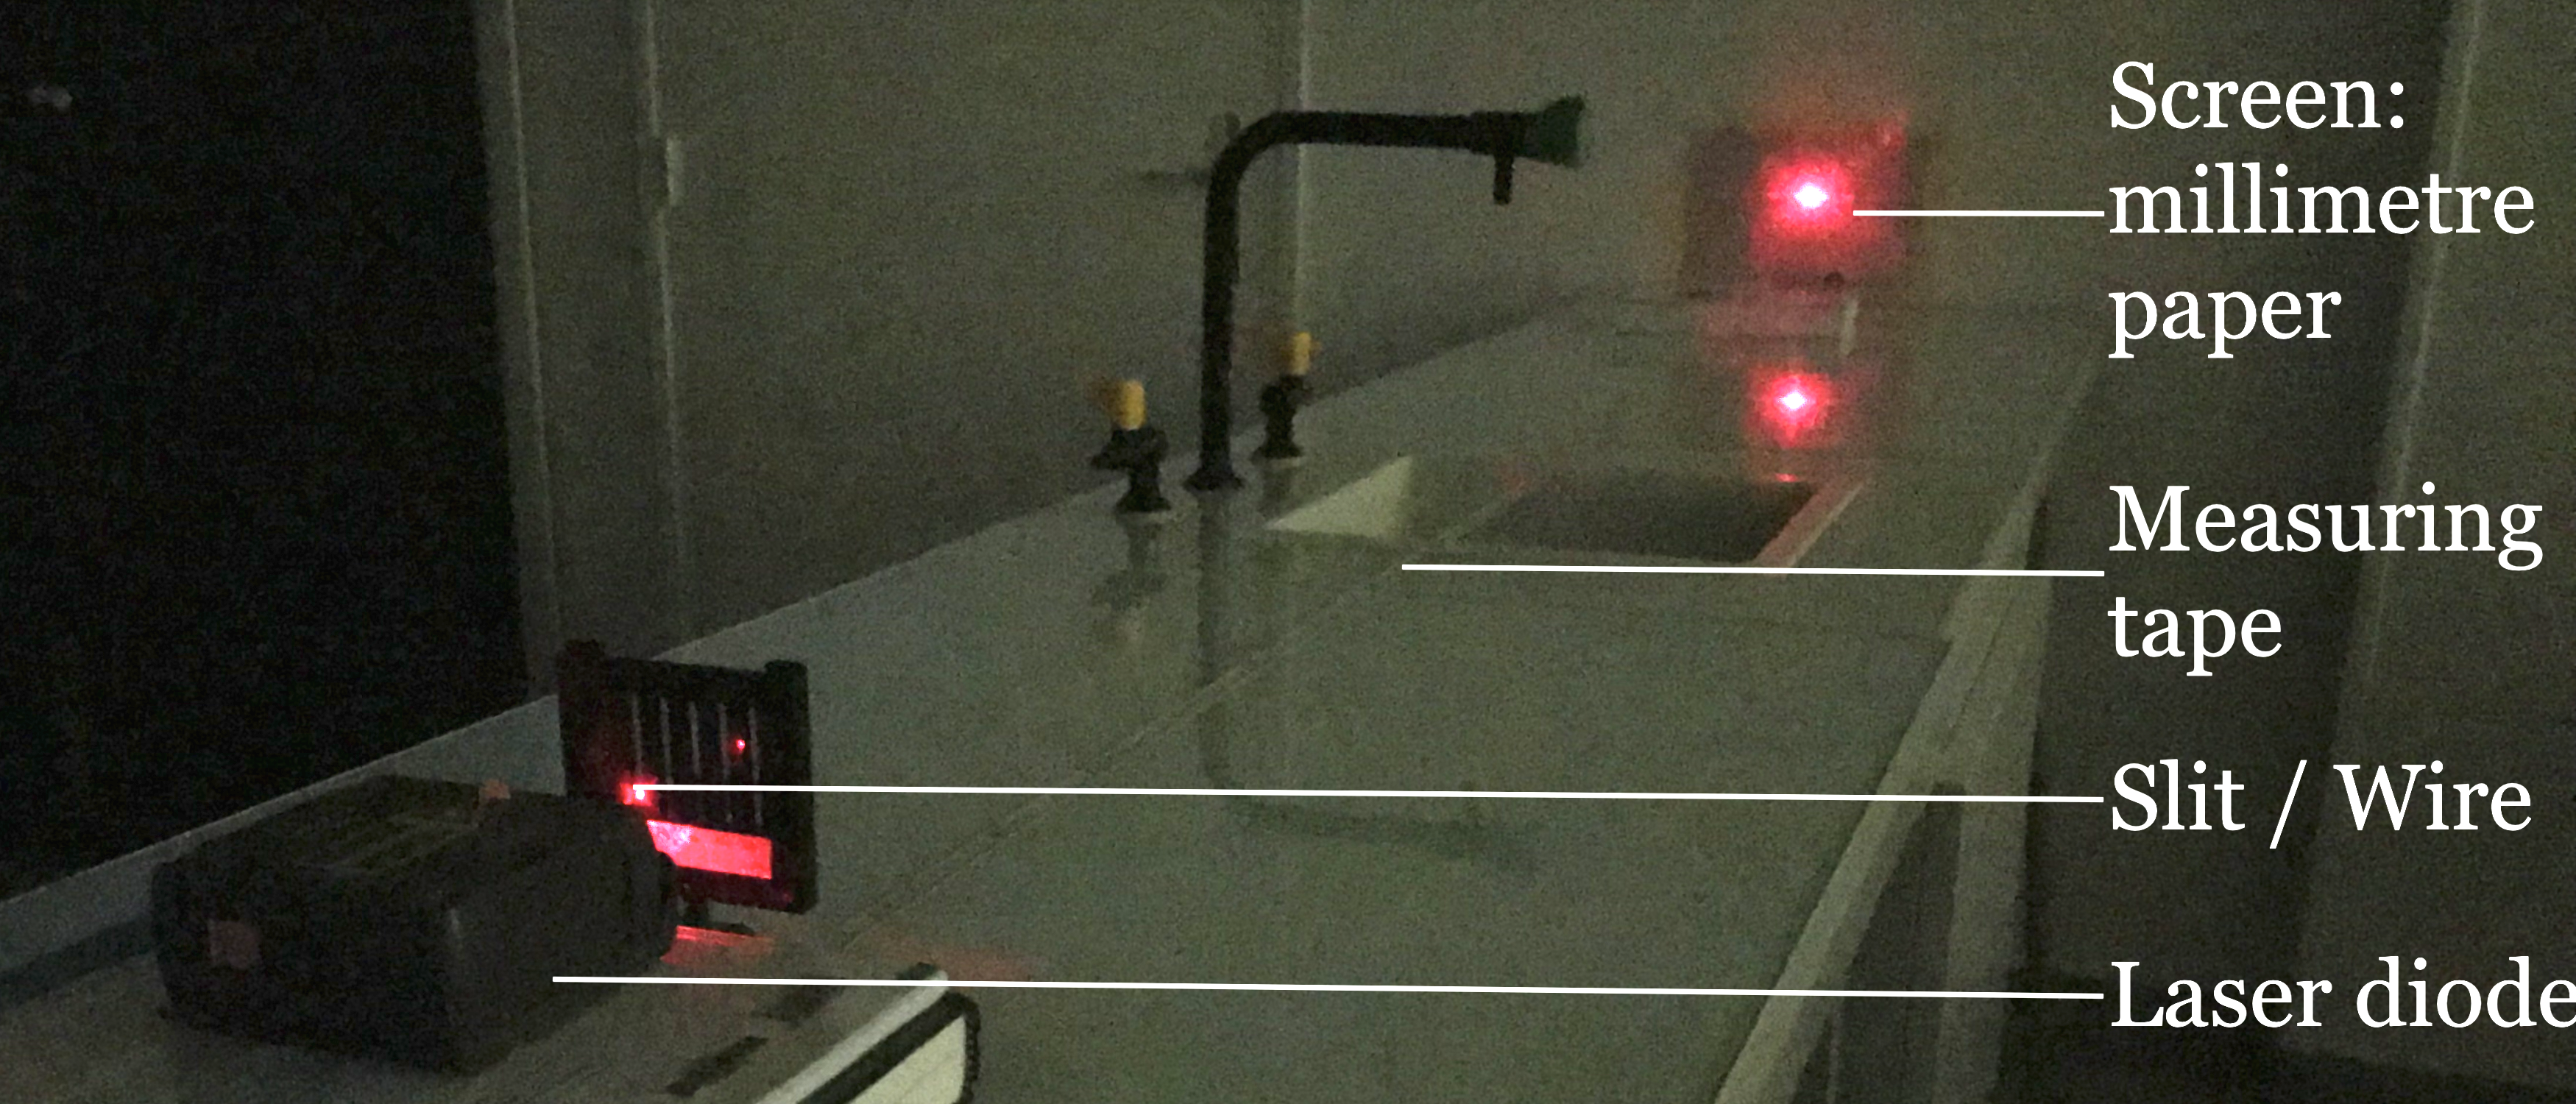
\includegraphics[width=\textwidth]{img/setup}
    \caption{Setup of the experiment; exposure modified for better visibility}
    \label{fig:setup}
\end{figure}
    \item Tape a piece of millimetre paper on the wall, aligning the centre of the paper with the laser beam while avoiding looking into the laser beam.
    \item Take a photo of the millimetre paper on which the diffraction pattern is observed. \label{step:get-pattern}
    \item Move the stand so that another wire of a different diameter is obstructing the laser beam. Make sure that the distance between the wires and the wall remains to be \SI{2.250+-0.010}{\m} (the uncertainty comes from the start and end). Repeat step \ref{step:get-pattern}. \label{step:change-wire}
    \item Repeat step \ref{step:change-wire} until the diffraction patterns of all 6 wires are recorded. \label{step:iterate-wire}
    \item Take the millimetre paper and the tapes off from the wall. Turn off the laser diode. \label{step:clean-up}
\end{enumerate}

\section{Raw Data}

\begin{figure}[H]
\centering
    \subfloat[\SI{38}{\um}]{
        \includegraphics[width=.984\textwidth]{img/wires/38}
    }
\end{figure}
\begin{figure}[H]
\ContinuedFloat
\centering
    \subfloat[\SI{50}{\um}]{
        \includegraphics[width=.984\textwidth]{img/wires/50}
    }    

    \subfloat[\SI{76}{\um}]{
        \includegraphics[width=.984\textwidth]{img/wires/76}
    }
    
    \subfloat[\SI{100}{\um}]{
        \includegraphics[width=.984\textwidth]{img/wires/100}
    }
    
    \subfloat[\SI{120}{\um}]{
        \includegraphics[width=.984\textwidth]{img/wires/120}
    }
    
    \subfloat[\SI{150}{\um}]{
        \includegraphics[width=.984\textwidth]{img/wires/150}
    }    
    \caption{Diffraction patterns produced by wires of varying diameters}
\end{figure}

The diffraction patterns produced are qualitatively akin to the ones from the single slit diffraction experiment. 
We observe a series of dark and bright fringes: 
there is a central bright fringe; 
the intensity of subsequent bright fringes decreases significantly. 
Overall, the width of bright diffraction fringes appears to decrease as the wire diameter increases. 

\section{Processed Data}
We provide a sample calculation below using a photo from the $d = \SI{100}{\um}$ trial.

In order to obtain $\Delta s$ in \cref{eq:hypothesis}, we first need to extract a 1D array of the relative intensities capturing the diffraction pattern from the 2D photo. 
This is achieved with a Python script \autocite{py_extract} by finding a line passing through all the diffraction fringes, as shown in \cref{fig:processed-axis}.

\begin{figure}[H]
    \includegraphics[width=\textwidth]{scripts/processed-data/axis}
    \caption{Line (in blue) passing through all the diffraction fringes}
    \label{fig:processed-axis}
\end{figure}

Since the laser beam is red, the BLUE and GREEN channels may be omitted, and only the RED channel of the image is considered. 
The diffraction pattern is then represented by an array of values between 0 and 255 --- with 0 corresponding to black and 255 corresponding to the brightest saturated red --- for each pixel along the line. 

Before proceeding to calculate an average value of $\Delta s$ for this photo, we first want to convert the fringe width from pixels to millimetres. 
This is where the millimetre paper comes into play. 
By convention, we define the top left corner of the image to be of pixel coordinates $(0, 0)$. 
A point on the millimetre paper occupies a square whose 2 opposite corners are at $(2375, 71)$ and $(2381, 75)$; 
i.e., this point's pixel coordinates are $(2378 \pm 3, 73 \pm 2)$. 
In the same manner, it is determined that another point which is \SI{20.0}{\mm} horizontally and \SI{1.0}{\mm} vertically apart on the millimetre paper has pixel coordinates of $(2660 \pm 3, 60 \pm 2)$. 
In other words, 
\[ \sqrt{20.0^2 + 1.0^2} = \SI{20.0}{\mm} \]
on the millimetre paper is equivalent to a pixel distance of
\[ \sqrt{ (2378 - 2660)^2 + (73 - 60)^2 } = \SI{282}{\px}; \]
i.e., $\SI{1}{\px} = \SI{0.0709}{\mm}$ with $0.0709 = 20 / 282$.
We will not present the derivation of the associated uncertainty, since it becomes apparent later that the uncertainty of \SI{+-2.19}{\%} can be safely ignored due to more significant standard deviations.

Now that we have converted the position from pixels to millimetres, we need to calculate the widths of diffraction fringes from the positions of the minima. 
As shown in \cref{fig:intensity}, the experimental data contain some significant noises, especially in the region of the central bright fringe. 

\begin{figure}[H]
    \includegraphics[width=\textwidth]{scripts/processed-data/intensity}
    \caption{Variation of pixel intensity across the diffraction pattern}
    \label{fig:intensity}
\end{figure}

To overcome this, we applied the Savitzky-Golay filter \autocite{scipy_smooth_filter} and programmatically detected the minima after smoothing the data. 
The average width of diffraction fringes for this photo of the $d = \SI{100}{\um}$ trial is then calculated to be \SI{16.0+-1.1}{\mm}, where \SI{+-1.1}{\mm} is the standard deviation.

Repeating the above procedure for all the other photos, we obtain the following figures:

\begin{table}[H]
    \centering
    \caption{Fringe width versus wire diameter}
    \begin{tabular}{ |c|c|c| }
        \hline
        \textbf{Wire diameter $d$} (\si{\um}) &
        \textbf{Average fringe width $\Delta s$} (\si{\mm}) \\
        \hline
\num{ 38 } & \num{ 39.5 (11) } \\ \hline
\num{ 50 } & \num{ 29.6 (15) } \\ \hline
\num{ 76 } & \num{ 20.4 (9) } \\ \hline
\num{ 100 } & \num{ 16.0 (11) } \\ \hline
\num{ 120 } & \num{ 13.4 (8) } \\ \hline
\num{ 150 } & \num{ 10.8 (7) } \\ \hline
    \end{tabular}
\end{table}

The experimental data suggest an inversely proportional relationship between $d$ and $\Delta s$, as shown in \cref{fig:ds_vs_d}.

\begin{figure}[H]
    \centering
    \includegraphics[width=\textwidth]{scripts/processed-data/ds_vs_d}
    \caption{Average measured fringe width against wire diameter}
    \label{fig:ds_vs_d}
\end{figure}

We then linearise the data by plotting $\Delta s$ against $\dfrac{1}{d}$:

\begin{figure}[H]
    \centering
    \includegraphics[width=\textwidth]{scripts/processed-data/ds_vs_d_lin}
    \caption{Average fringe width against reciprocal of wire diameter} 
    \label{fig:ds_vs_d_lin}
\end{figure}

As shown in \cref{fig:ds_vs_d_lin}, the gradient of the best fit line is equal to $1439 \frac{\si{\mm}}{\si{\per\um}} = \SI{1439}{\nm \m}$; 
gradients of reasonable fit lines vary between \SI{1369}{\nm \m} and \SI{1550}{\nm \m}.

\section{Analysis}
\Cref{eq:hypothesis} can be rewritten as
\begin{align}
    \overbrace{\Delta s}^{y} 
    = 
    \underbrace{(\lambda D)}_{\text{gradient}} \times \overbrace{\frac{1}{d}}^{x}.
\end{align}
The uncertainty in the gradient of the best fit line in \cref{fig:ds_vs_d_lin} is \[\frac{1550 - 1369}{2} = \SI{90}{\nm \m}.\]
As such, $\lambda D = \SI{1439+-90}{\nm\m}$.
Since $D = \SI{2.250+-0.010}{\m}$ is a controlled variable,
\begin{align*}
    \lambda 
    &= \SI{1439}{\nm\m} / \SI{2.250}{\m}\\
    &= \SI{640}{\nm}
    .
\end{align*}

Since $\lambda = \text{gradient} / D$, we have concerning the uncertainties
\begin{align*}
    \fracDelta{\lambda} &= \fracDelta{\text{gradient}} + \fracDelta{D}\\
    &= \frac{90}{1439} + \frac{0.010}{2.250}\\
    &= \SI{6.8}{\%}.
\end{align*}
The absolute uncertainty in $\lambda$ is then
\begin{align*}
    \Delta \lambda = 6.8\% \times \SI{640}{\nm} = \SI{+-42}{\nm}.
\end{align*}

Regarding the laser wavelength $\lambda$, the experimentally determined value \SI{640+-42}{\nm} is coherent with the manufacturer's value of \SI{650+-10}{\nm} \autocite{laser-specs}.
There is a percentage error of 
\begin{align*}
    &\frac{\lambda_\text{accepted} - \lambda_\text{experimental}}{\lambda_\text{accepted}}\\
    &= \frac{650 - 640}{640}\\
    &= 1.5\%
\end{align*}

Since the percentage error of \SI{1.5}{\%} is less than the percentage uncertainty of \SI{6.8}{\%}, the experiment is valid within the limits of the apparatus used.
Nevertheless, the non-null y-intercept of \SI{+1.37}{\mm} of the best fit line in \cref{fig:ds_vs_d_lin} indicates that there are some systematic errors, which we will discuss below.

\section{Conclusion}
The experiment has shown that obstructing a monochromatic laser light with a thin wire produces a similar pattern to that of single slit diffraction. 
Moreover, the relationship between the wire diameter and the width of diffraction fringes can be described by \cref{eq:hypothesis}, which is in fact the same equation for fringe width in the case of single slit diffraction.
Babinet's principle accounts for this phenomenon \autocite{babinet}:
\begin{quote}
    ``Suppose that the eye observes a point source of light.
    If a small opaque object is placed just off the line of sight, the effect of this object is the same as that of a precisely similar aperture illuminated from the same source.''
\end{quote}

\section{Evaluation}
At last, we shall address the random and systematic errors in the experiment.

To start with, the measured value of $D$ represents the distance between the stand and the wall and not the actual distance from the wire to the screen:
at one end, the measurement starts from the edge of the stand instead of the actual exact position of the wires, which is closer to the screen; 
at the other end, the millimetre paper is not mounted perfectly flat to the wall.
Consequently, the measured value of $D$ is greater than the actual value.
Since we calculate the laser wavelength using $\lambda = \text{gradient} / D$, the experimentally determined value of $\lambda$ will be smaller than the actual value. Together with the uncertainty of \SI{+-10}{\nm} in the manufacturer's value \autocite{laser-specs}, this accounts for the discrepancy between the calculated value of \SI{640}{\nm} and the accepted value of \SI{650}{\nm}.
The straightforward solution is to measure the distance between the exact positions of the wire and the screen.
However, due to the practical difficulties, it is much more favourable to simply increase $D$ so that the inaccuracy becomes less significant. 
In doing so, we also decrease the fractional uncertainty in $D$, and as such reduce the uncertainty of \SI{6.8}{\%} in $\lambda$ making the results more precise.

Another systematic error arises from determining the locations of destructive interference. 
As shown in \cref{fig:intensity}, there are significant noises in the unprocessed experimental data. 
Inevitably, the Savitzky-Golay filter that we applied to reduce these noises distorts the diffraction pattern: 
the minima in the data after smoothing are more spread out to the edges of the screen; 
this effect is more marked for fringes that are further away from the centre. 
Overall, the programmatically determined fringe widths are greater than the actual widths. 
The positive y-intercept of the best fit line in \cref{fig:ds_vs_d_lin} reflects this systematic error. 
One solution is to use a high-quality laser and a high-resolution charge-coupled device as the screen to record the intensity in the diffraction pattern with high precision. 
This method is nonetheless costly, since the equipment usually is not available in a school laboratory. 
Another more practical solution is proposed by Wu et al.\ \autocite{fourier} in 2015 using Fourier transform, an alternative mathematical method to process the experimental intensity data without degrading the accuracy.

An advantage of the experiment is that it is easy to set up with readily available materials, and the use of digital photo analysis allows rapid data collection and processing without introducing human errors. 
In spite of that, care must be taken to fix the position and angle of the camera to avoid distorting the photographed diffraction pattern and as such giving rise to important systematic errors.

One possible way to extend the experiment is to study the diffraction pattern when other types of thin obstacles such as filament or hair are used. 
The larger range of diameters helps improve the precision of the results.
The uncertainty of \SI{6.8}{\%} in $\lambda$ mostly results from the uncertainty in the gradient of the best fit line. 
Recall that the maximum gradient of an acceptable fit line is given by
\[ \frac{(y_{max} + \Delta y_{max}) - (y_{min} - \Delta y_{min})}{ x_{max} - x_{min} } 
= 
\overbrace{\frac{y_{max} - y_{min}}{x_{max} - x_{min}}}^{\text{slope of best fit line}} + \overbrace{\frac{\Delta y_{max} + \Delta y_{min} }{x_{max} - x_{min}}}^{\text{uncertainty in slope}}. \]
As long as the uncertainties in the average fringe width $\Delta y_{max}$ and $\Delta y_{min}$ do not become much more significant as the diameter becomes very small or very big, a greater value of $x_{max} - x_{min}$ decreases the uncertainty in the gradient. 
By using \cref{eq:hypothesis}, we can then extrapolate the diameter of an unknown obstacle with high precision from the width of diffraction fringes produced. 
This has been applied in real life to accurately measure the size of red blood cells using optical diffraction. \autocite{blood_cell_success}

\printbibliography

\end{document}
